% --- Template for thesis / report with tktltiki2 class ---
% 
% last updated 2013/02/15 for tkltiki2 v1.02

\documentclass[12pt,finnish]{tktltiki2}

% tktltiki2 automatically loads babel, so you can simply
% give the language parameter (e.g. finnish, swedish, english, british) as
% a parameter for the class: \documentclass[finnish]{tktltiki2}.
% The information on title and abstract is generated automatically depending on
% the language, see below if you need to change any of these manually.
% 
% Class options:
% - grading                 -- Print labels for grading information on the front page.
% - disablelastpagecounter  -- Disables the automatic generation of page number information
%                              in the abstract. See also \numberofpagesinformation{} command below.
%
% The class also respects the following options of article class:
%   10pt, 11pt, 12pt, final, draft, oneside, twoside,
%   openright, openany, onecolumn, twocolumn, leqno, fleqn
%
% The default font size is 11pt. The paper size used is A4, other sizes are not supported.
%
% rubber: module pdftex

% --- General packages ---

\usepackage[utf8]{inputenc}
\usepackage[T1]{fontenc}
\usepackage{lmodern}
\usepackage{microtype}
\usepackage{amsfonts,amsmath,amssymb,amsthm,booktabs,color,enumitem,graphicx}
\usepackage[pdftex,hidelinks]{hyperref}

% Automatically set the PDF metadata fields
\makeatletter
\AtBeginDocument{\hypersetup{pdftitle = {\@title}, pdfauthor = {\@author}}}
\makeatother

% --- Language-related settings ---
%
% these should be modified according to your language

% babelbib for non-english bibliography using bibtex
\usepackage[fixlanguage]{babelbib}
\selectbiblanguage{finnish}

% add bibliography to the table of contents
\usepackage[nottoc]{tocbibind}
% tocbibind renames the bibliography, use the following to change it back
\settocbibname{Lähteet}

% spacing
\usepackage{setspace}
\onehalfspacing

% enumitem
\usepackage{enumitem}

% algorithm snippets
\usepackage{algorithm}
\usepackage{algpseudocode}
\usepackage{caption}
\floatname{algorithm}{Algoritmi}

% copy paste from http://tex.stackexchange.com/questions/33866/algorithm-tag-and-page-break
\DeclareCaptionFormat{algor}{%
  \hrulefill\par\offinterlineskip\vskip1pt%
    \textbf{#1#2}#3\offinterlineskip\hrulefill}
\DeclareCaptionStyle{algori}{singlelinecheck=off,format=algor,labelsep=space}
\captionsetup[algorithm]{style=algori}

% --- Theorem environment definitions ---

\newtheorem{lau}{Lause}
\newtheorem{lem}[lau]{Lemma}
\newtheorem{kor}[lau]{Korollaari}

\theoremstyle{definition}
\newtheorem{maar}[lau]{Määritelmä}
\newtheorem{ong}{Ongelma}
\newtheorem{alg}[lau]{Algoritmi}
\newtheorem{esim}[lau]{Esimerkki}

\theoremstyle{remark}
\newtheorem*{huom}{Huomautus}


% --- tktltiki2 options ---
%
% The following commands define the information used to generate title and
% abstract pages. The following entries should be always specified:

\title{Monte Carlo -puuhaku ja pelitekoälyt}
\author{Kalle Viiri}
\date{\today}
\level{Kandidaatintutkielma}
\abstract{Monte Carlo -puuhaku (\textit{Monte Carlo Tree Search}) on puuhakualgoritmi, jota on käytetty pelitekoälyissä lupaavin tuloksin erityisesti gon saralla. Menetelmä korvaa perinteisen \textit{minimax}-haun kanssa tyypillisesti käytetyn heuristiikan satunnaistetulla simuloinnilla osittaisessa pelipuussa. Tämä mahdollistaa menetelmän käyttämisen myös peleissä, joihin ei tunneta hyviä heuristiikkoja.

Puuhaun toteutuksen tehokkuus riippuu paljon simuloitavien solmujen valinnasta. Suosituin Monte Carlo -puuhaun toteutus, puiden luottamusylärajamenetelmä, hyödyntää aikaisempaa tutkimusta monikätisen rosvon ongelmasta (\textit{multi-armed bandit problem}) ja siihen kehitetystä luottamusylärajamenetelmästä valitakseen simuloitavat solmut tehokkaasti niiden odotusarvon perusteella.

Monte Carlo -puuhaun vahvuus pelitekoälynä kasvaa käytettävissä olevan laskenta-ajan kasvaessa. Haku on kuitenkin katkaistavissa tai aikarajattavissa, jolloin sitä voi soveltaa kombinatoristen pelien lisäksi myös reaaliaikaisiin peleihin. Sopivien determinisaatiotekniikoiden avulla menetelmää voi soveltaa myös peleihin, joissa esiintyy satunnaistekijöitä tai epätäydellistä informaatiota.}

% The following can be used to specify keywords and classification of the paper:

\keywords{Monte Carlo, puuhaku, tekoäly}

% classification according to ACM Computing Classification System (http://www.acm.org/about/class/)
% This is probably mostly relevant for computer scientists
% uncomment the following; contents of \classification will be printed under the abstract with a title
% "ACM Computing Classification System (CCS):"
\classification{
\\\textbf{Computing methodologies---Randomized search}
\\\textit{Computing methodologies--Game tree search}
}

% If the automatic page number counting is not working as desired in your case,
% uncomment the following to manually set the number of pages displayed in the abstract page:
%
% \numberofpagesinformation{16 sivua + 10 sivua liitteissä}
%
% If you are not a computer scientist, you will want to uncomment the following by hand and specify
% your department, faculty and subject by hand:
%
% \faculty{Matemaattis-luonnontieteellinen}
% \department{Tietojenkäsittelytieteen laitos}
% \subject{Tietojenkäsittelytiede}
%
% If you are not from the University of Helsinki, then you will most likely want to set these also:
%
% \university{Helsingin Yliopisto}
% \universitylong{HELSINGIN YLIOPISTO --- HELSINGFORS UNIVERSITET --- UNIVERSITY OF HELSINKI} % displayed on the top of the abstract page
% \city{Helsinki}
%


\begin{document}
% --- Front matter ---

\frontmatter      % roman page numbering for front matter

\maketitle        % title page
\makeabstract     % abstract page

\tableofcontents  % table of contents

% --- Main matter ---

\mainmatter       % clear page, start arabic page numbering

\section{Johdanto}

\subsection{Peliteoria ja pelipuu}

Pelillä tarkoitetaan peliteoriassa ongelmaa, jossa yksi tai useampi toimija vaikuttavat päätöksillään lopputulokseen, jolla on jokin määritelty arvo kullekin pelaajista~\cite{browne}. Mahdollisten pelitilanteiden joukkoa merkitään $S$. Pelillä on alkutila $s_0 \in S$ ja joukko lopputiloja $S_T \subseteq S$. Mahdollisten siirtojen joukkoa merkitään $A$:lla, ja tilasiirtymäfunktio $f : S \times A \rightarrow S$ määrittää, mihin tilaan päädytään lähtötilasta milläkin siirrolla.

Pelin lopputuloksen edullisuus pelaajalle määritellään palkintofunktiolla $R : S \rightarrow \mathbb{R}$. Tässä tekstissä käytetään usein käytettyä palkintofunktiota, joka on arvoltaan $0$ pelitilanteissa jotka eivät ole lopputilanteita, ja lopputilanteille $1$ voittavista tilanteista, $0$ tasapeleistä ja $-1$ häviöistä.

Kahden pelaajan peli on kombinatorinen, kun se täyttää seuraavat ehdot~\cite{browne}:

\begin{enumerate}[label=\roman*.]
	\item Nollasummaisuus, eli jokaisessa tilassa pelaajien palkintofunktioiden summa on nolla. Tämä tarkoittaa, että yhden pelaajan parantaessa tulostaan toisen pelaajan tulos heikkenee.
	 \item Täydellinen informaatio, eli tarkka pelitilanne on jatkuvasti molempien pelaajien tiedossa.
	 \item Determinismi, eli peliin ei sisälly satunnaistekijöitä.
	 \item Vuorottaisuus, eli pelaaja voi toiminnallaan vaikuttaa pelitilanteeseen vain määrätyillä vuoroillaan.
	 \item Diskreetti, eli peliä pelataan erillisissä vuoroissa reaaliaikaisuuden sijaan.
\end{enumerate}

Esimerkkejä kombinatorisista peleistä ovat shakki ja go. Kombinatoriset pelit ovat tekoälylle erinomainen tutkimus- ja soveltamisala, sillä niissä on usein yksinkertaiset säännöt, joiden päälle rakentuu kuitenkin edistynyttä strategiaa~\cite{browne}.

Kombinatorinen peli on helppo mallintaa pelipuuna. Pelipuun juurisolmu kuvaa pelin alkutilannetta ja jokaisen solmun lapset pelitilanteita, jotka solmun kuvaamasta pelitilanteesta voi saavuttaa. Pelipuun lehtisolmut ovat lopputilanteita, joissa pelin lopputulos määräytyy. Pelipuuna mallinnettua peliä voi käsitellä tavallisilla puuhakualgoritmeilla~\cite{aima}.

\subsection{Minimax ja heuristiikka}

Perinteinen tapa toteuttaa pelitekoälyjä on minimax-haku, jossa tekoäly olettaa kaikkien pelaajien pyrkivän maksimoimaan oman voittonsa toisten pelaajien pelatessa optimaalisesti~\cite{aima}. Tällainen tekoäly valitsisi siis mieluummin varmasti tasapeliin johtavan siirron kuin sellaisen, jolla voi vastustajan valinnoista riippuen joko voittaa tai hävitä. Lopputulosta, joka seuraa kun molemmat pelaajat pelaavat minimax-strategian mukaan tietystä tilanteesta, kutsutaan tilanteen minimax-arvoksi.

Minimax-haun ongelmana on se, että vain puun lehtisolmujen arvo on tiedossa pelaajille~\cite{aima}. Yksinkertaisissa peleissä, kuten 3x3-ristinollassa, tämä ei ole vielä ongelma, mutta vaikkapa shakin pelipuu haarautuu aivan liian runsaasti, jotta hakua voitaisiin jatkaa lehtisolmuihin asti. Jotta seuraava siirto saataisiin valittua järkevässä ajassa, on haku katkaistava ennen pelin lopputilanteisiin pääsemistä. Koska haku ei välttämättä pääse pelin lopputilanteisiin saakka, se tarvitsee keinon arvioida keskeneräisten pelien minimax-arvoa.

Keskeneräisen pelitilanteen perusteella minimax-arvoa arvioivaa funktiota kutsutaan heuristiikaksi. Yksinkertainen heuristiikka shakkiin voi olla esimerkiksi nappuloiden lukumäärän laskeminen. Tätä heuristiikkaa käyttävä tekoäly osaisi valita tilanteita, joissa se saa materiaalietumatkaa, mutta edistyneemmät heuristiikat osaisivat painottaa tilanteita myös nappuloiden arvon ja sijainnin mukaan. Heuristiikkojen ongelmana on, että hyvän heuristiikan muodostaminen vaatii kehittäjältään paljon ymmärrystä pelistä. Joihinkin peleihin, esimerkiksi gohon, ei tunneta heuristiikkoja, joilla tekoäly olisi kilpailukykyinen vahvoja ihmispelaajia vastaan~\cite{browne}.


\section{Monte Carlo -puuhaku}

Monte Carlo -puuhaku (\textit{Monte Carlo Tree Search}, jatkossa MCTS)~\cite{browne} on puuhakumenetelmä, jossa heuristiikan sijaan pelitilanteita arvioidaan simuloimalla niistä satunnaisotannalla pelejä lopputilanteeseen asti. Kukin solmu hyödyntää kauttaan kulkeneita simulaatioita muodostaakseen arvion todellisesta minimax-arvostaan. Perusajatuksena on, että simuloitujen pelien määrän kasvaessa odotusarvo tarkentuu vastaamaan niiden lähtötilanteen totuudenmukaista minimax-arvoa.

MCTS-menetelmässä pelipuuta rakennetaan iteratiivisesti tarpeen mukaan. Haku aloitetaan pelipuulla, jossa on pelkästään pelin alkutilaa $s_0$ vastaava solmu $v_0$. Puuta laajennetaan kulkemalla juuresta alkaen puussa alaspäin. Kuljettavan haaran valinta on toteutusriippuvaista, mutta useimmat toteutukset pyrkivät laajentamaan haaroja joista on jo saatu hyviä tuloksia. Kun saavutaan solmuun, jolla on pelipuuhun liittämättömiä lapsia, voidaan joko jatkaa etenemistä puuhun jo liitettyihin lapsiin tai valita tämänhetkinen solmu laajennettavaksi solmuksi.

Kun laajennettava solmu on valittu, puuhun liitetään sen uudeksi lapseksi jokin siitä seuraava pelitilanne. Tästä lapsesta suoritetaan pelin loppuun päättyvä simulaatio, jossa molempien pelaajien vuorot pelataan satunnaisilla siirroilla~\cite{browne}. Pelin lopettavaan tilanteeseen päädyttäessä simulaatio voi tarkistaa pelin voittoehdoista lopputuloksen $\Delta$. Saatu $\Delta$ palautetaan pelipuussa vastavirtaan juureen asti. Matkalla olevien solmujen odotusarvoja päivitetään uuden $\Delta$-arvon mukaan, jolloin solmuille muodostuu simulaatioiden määrän kasvaessa jatkuvasti tarkempi arvio solmun todellisesta minimax-arvosta.~\cite{browne}.

\begin{figure}

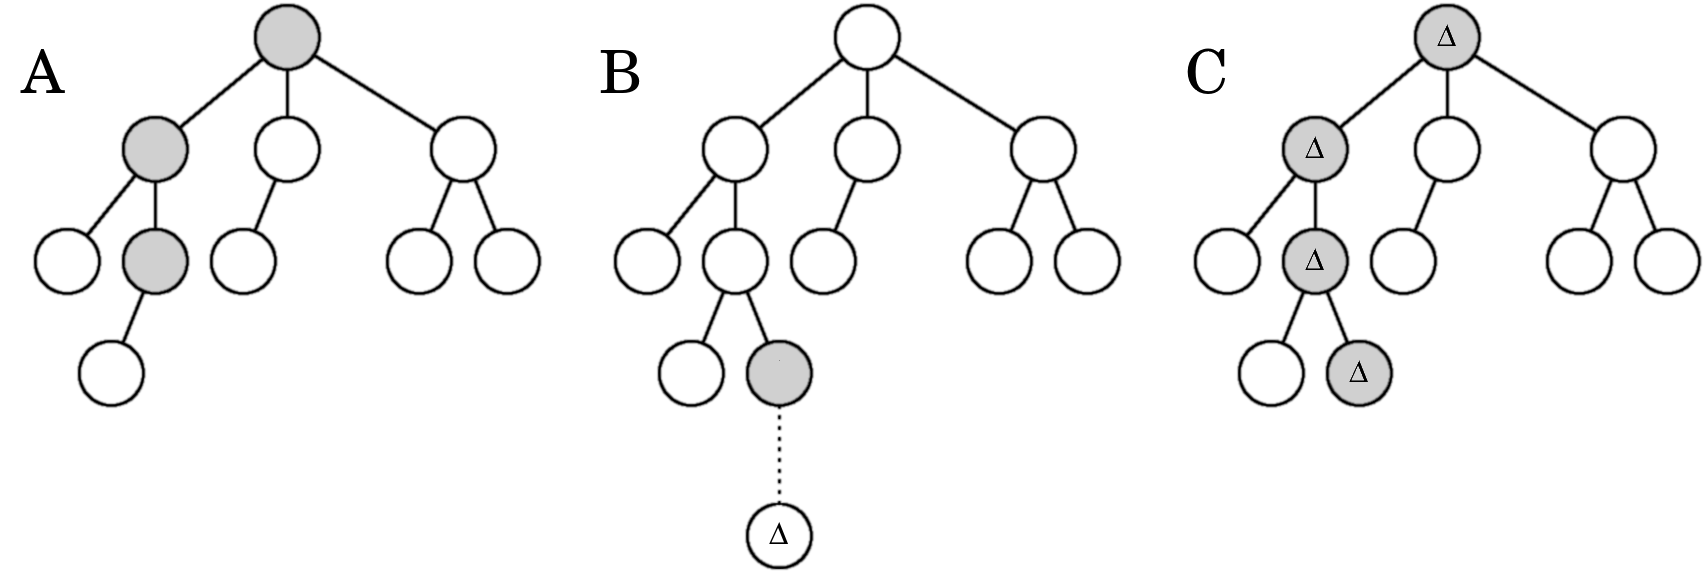
\includegraphics[width = \textwidth]{basicmcts.png}

\caption{MCTS:n vaiheet. A: Laajennettavan solmun valinta pelipuusta. B:~Uuden solmun lisääminen ja simulaatio. C: Odotusarvojen päivittäminen vastavirtaan simulaation perusteella.}
\end{figure}


Algoritmissa \ref{MCTS} esitellään Brownen ym. yleistetty MCTS~\cite{browne}. Aliohjelmien \textsc{ValitseLapsi}, \textsc{Simuloi}, \textsc{Vastavirta} ja \textsc{ParasLapsi} toiminta on jätetty kuvaamatta, sillä ne vaihtelevat erilaisten MCTS-toteutusten välillä. Esimerkkitoteutus näille esitellään algoritmissa \ref{UCT}.

\newpage
\begin{samepage}
\begin{center}
\captionof{algorithm}{Yleistetty MCTS}
\label{MCTS}
\begin{algorithmic}[0]
\Function{MctsHaku}{$s_0$}
	\State luo pelipuun juuri $v_0$ pelitilanteesta $s_0$
	\While{laskenta-aikaa on jäljellä}
		\State $v_1 \leftarrow$ \Call{ValitseLapsi}{$v_0$}
		\State $\Delta \leftarrow$ \Call{Simuloi}{$s(v_1)$}
		\State \Call{Vastavirta}{$v_1$, $\Delta$}
	\EndWhile
	\State \Return siirto(\Call{ParasLapsi}{$v_0$})
\EndFunction
\end{algorithmic}
\rule{\textwidth}{1pt}
\end{center}
\end{samepage}

Hakua jatketaan niin kauan kuin laskenta-aikaa riittää tai kunnes suoritus katkaistaan ulkopuolelta. Haun päätyttyä valitaan siirto, joka katsotaan haun aloitustilanteesta suoritettujen simulaatioiden perusteella parhaaksi. Parhaan siirron valintaan mahdollisista siirroista on useita malleja~\cite{browne}. Yksi yleinen ratkaisu on valita lapsi, jolla on korkein odotusarvo. Odotusarvo on kuitenkin usein harhaanjohtava solmuille, joita on simuloitu vain vähän, joten toinen suosittu malli on valita solmu jota on simuloitu eniten.

\section{UCT-menetelmä}

\subsection{Monikätisen rosvon ongelma}

Monikätisen rosvon optimointiongelmassa (\textit{multi-armed bandit problem})~\cite{browne} pelaajalla on peliautomaatti, jossa on $K$ vipua. Jokaiselle vivulle on määritelty pelaajalle tuntematon todennäköisyysjakauma, jonka mukaan pelaaja saa palkinnon vetäessään vipua. Ongelmana on löytää strategia, jolla minimoidaan pelkästään parasta vipua pelaavan strategian kokonaispalkinnon etumatka omaamme nähden.

Tehokkaan pelistrategian löytäminen monikätisen rosvon ongelmaan edellyttää algoritmia, joka osaa pelata paljon vivuilla joista on jo saatu hyviä tuloksia. Samalla kuitenkin sen on tutkittava välillä muitakin vipuja, jotta mahdollisesti huomaamatta jääneet paremmat vivut voidaan hyödyntää. Valintatilannetta aikaisemmin hyviä tuloksia antaneiden vaihtoehtojen ja parempien vaihtoehtojen etsimisen vähemmän tutkituista vivuista kutsutaan tutkimus-hyödyntämis -dilemmaksi (\textit{exploration-exploitation dilemma}).

Dilemman ratkaisevan strategian esittelevät Auer ym. joiden luottamusylärajan menetelmä~\cite{auer} (\textit{Upper Confidence Bounds}, jatkossa UCB1) valitsee pelattavaksi vivun joka maksimoi lausekkeen
\begin{equation}
\text{UCB1} = \overline{X}_j + \sqrt{\frac{2 \ln n}{n_j}}
\end{equation}
arvon, missä $X_j$ on vivun $j$ tuottamien palkintojen keskiarvo, $n_j$ on vivun $j$ pelikertojen määrä tähän mennessä ja $n$ on koko pelikoneen pelikertojen määrä. Tasapelit ratkaistaan toteutuksissa tyypillisesti satunnaisesti, ja kun $n_j = 0$ katsotaan että $\text{UCB1} = \infty$ eli kaikkia vipuja kokeillaan vähintään kerran ennen kuin yhtäkään pelataan toista kertaa~\cite{browne}.

Lai ja Robbins~\cite{lai} osoittivat, että useille palkintojakaumille ei ole olemassa monikätisen rosvon pelistrategiaa, jossa ainoastaan parasta vipua pelaavan strategian etumatka kasvaa hitaammin kuin $O(\ln n)$. UCB1:lla optimaalisen strategian etumatka kasvaa logaritmisesti, joten sitä voi pitää hyvänä ratkaisuna monikätisen rosvon ongelmaan. Se on myös yksinkertainen ja tehokas~\cite{browne}, joten se on mielekäs ratkaisu sovellettavaksi toisiin ongelmiin, kuten puun laajentamiseen MCTS:ssä.

\subsection{Luottamusylärajat puuhaussa}

Kocsisin ja Szepesvárin~\cite{kocsis} esittelemä puuhakujen luottamusyläraja -menetelmä (\textit{Upper Confidence Bounds for Trees} jatkossa UCT) on yleisimpiä algoritmeja MCTS:n toteutukseen. UCT mallintaa pelipuuta laajentaessa solmun valinnan monikätisen rosvon ongelmana, ja käyttää pelistrategiana muunnelmaa UCB1:stä. Tällöin $X_j$ on solmun $j$ kautta suoritettujen simulaatioiden lopputulosten keskiarvo, $n_j$ solmun $j$ läpi suoritettujen simulaatioiden lukumäärä ja $n$ kaiken kaikkiaan suoritettujen simulaatioiden lukumäärä.

UCB1:sta poiketen algoritmille annetaan tutkimusvakio (\textit{exploration term}) $C_p$ joka vaikuttaa algoritmin painotukseen uusien vaihtoehtojen tutkimuksen ja hyväksi tunnettujen hyödyntämisen välillä. Edetessään pelipuussa UCT pyrkii maksimoimaan lausekkeen
\begin{equation}
\text{UCT} = \overline{X}_j + C_p \sqrt{\frac{2 \ln n}{n_j}}
\end{equation}
arvon. Browne ym. esittelee UCT-haun algoritmin \ref{UCT} mukaisesti~\cite{browne}. Algoritmissa $s(v)$ on solmun $v$ kuvaama pelitilanne, $f(s(v), a)$ on tilanteesta $s(v)$ siirrolla $a$ saavutettava pelitilanne, $Q(v)$ on $v$:n kautta saavutetun palkinnon kokonaisarvo, $N(v)$ on $v$:n kautta kulkeneiden simulaatioiden lukumäärä ja $\Delta(v, p)$ on pelaajan $p$ palkintoarvo solmussa $v$. Algoritmi palauttaa siirron lapseen jolla on paras odotusarvo korvaamalla tutkimusvakion $C_p$ arvolla $0$.

\newpage

\begin{center}
\captionof{algorithm}{UCT-algoritmi}
\label{UCT}
\begin{algorithmic}[0]
\begin{samepage}
\Function{UctHaku}{$s_0$}
	\State luo pelipuun juuri $v_0$ pelitilanteesta $s_0$
	\While{laskenta-aikaa on jäljellä}
		\State $v_1 \leftarrow$ \Call{ValitseLapsi}{$v_0$}
		\State $\Delta \leftarrow$ \Call{Simuloi}{$s(v_1)$}
		\State \Call{Vastavirta}{$v_1$, $\Delta$}
	\EndWhile
	\State \Return siirto(\Call{ParasLapsi}{$v_0, 0$})
\EndFunction
\end{samepage}
\\
\\
\begin{samepage}
\Function{ValitseLapsi}{$v$}
	\While{$v$ ei ole lehti}
		\If{$v$:llä on puuhun lisäämättömiä lapsia}	
			\State \Return \Call{Laajenna}{$v$}
		\Else
			\State $v \leftarrow$ \Call{ParasLapsi}{$v, C_p$}
		\EndIf
	\EndWhile
	\State \Return{$v$}
\EndFunction
\end{samepage}
\\
\begin{samepage}
\Function{Laajenna}{$v$}
	\State valitse $a$ joka on tutkimaton siirto tilasta $s(v)$
	\State lisää $v$:lle lapsi $v'$ siten että $s(v') = f(s(v), a)$
	\State \Return $v'$
\EndFunction
\end{samepage}
\\
\begin{samepage}
\Function{ParasLapsi}{$v, c$}
	\State \Return $v$:n lapsi jolla on suurin $\frac{Q(v')}{N(v')} + c\sqrt{\frac{2 \ln N(v)}{N(v')}}$
\EndFunction
\end{samepage}
\\
\begin{samepage}
\Function{Simuloi}{$s$}
	\While{$s$ ei ole pelin lopputilanne}
		\State valitse $a \in A(s)$ satunnaisesti tasajakaumalla
		\State $s \leftarrow f(s, a)$
	\EndWhile
	\State \Return $R(s)$ 
\EndFunction
\end{samepage}
\\
\begin{samepage}
\Function{Vastavirta}{$v, \Delta$}
	\While{$v$ ei ole \textit{null}}
		\State $N(v) \leftarrow N(v) + 1$
		\State $Q(v) \leftarrow Q(v) + \Delta(v, p)$
		\State $v \leftarrow v$:n vanhempi
	\EndWhile
\EndFunction
\end{samepage}
\end{algorithmic}
\rule{\textwidth}{1pt}
\end{center}


\section{Parannuksia menetelmään}

\subsection{Vahvat ja tasapainoiset simulaatiot}

Tavallinen MCTS-toteutus käy simulaatiovaiheen läpi satunnaisilla siirroilla~\cite{browne}. Satunnaisten siirtojen mallin etuja ovat toteutuksen yksinkertaisuus ja mahdollisten tutkittavien tilanteiden monipuolisuus. Satunnaiset siirrot eivät kuitenkaan mallinna hyvin oikeiden pelaajien tekemiä ratkaisuja, joten simulaatiovaiheen tulokset eivät välttämättä kuvaa tilan todellista arvoa. Eroa tilan odotusarvon ja sen todellisen minimax-arvon välillä kutsutaan simulaation virheeksi (\textit{error})~\cite{silver}.

Gelly ja Silver~\cite{gellysilver} käsittelevät artikkelissaan simulaatiomalleja, jotka pyrkivät minimoimaan kunkin suoritetun simulaation virheen hyödyntämällä heuristiikkaa tai koneoppimismenetelmiä, eli vahvoja simulaatioita. Koska MCTS:n toimivuus perustuu simulaatiokertojen määrään, vahvojen simulaatioiden on pystyttävä hyvien siirtojen tekemisen lisäksi toimimaan nopeasti, jotta otoskoko pysyy tarpeeksi suurena~\cite{browne}.

Silver ja Tesauro~\cite{silver} käsittelevät vahvojen simulaatioiden ominaisuuksia ja toteavat, että vahva simulaatio voi jopa heikentää MCTS:n tehokkuutta. Vahvat simulaatiot ovat helposti liian deterministisiä, jolloin pienet, systemaattiset virheet yksittäisissä simulaatioissa kasaantuvat usean simulaation aikana suureksi poikkeamaksi todellisesta minimax-arvosta.

Silver ja Tesauro toteavat, että virheen minimoinnin sijasta on järkevää minimoida kokonaisvirheen odotusarvo~\cite{silver}. Tällaista mallia noudattavan simulaation annetaan synnyttää virhettä, mutta virheen suunta pyritään tasaamaan siten, että liian optimistisia virhearvioita syntyy samassa suhteessa kuin liian negatiivisia. Yltiöoptimistiset ja -pessimistiset virheet siis tasaavat toisensa pois, jolloin kokonaisarvio on lähellä todellista minmax-arvoa. Silver ja Tesauro kutsuvat kokonaisvirheen odotusarvoa minimoimaan pyrkivää simulaatiomallia tasapainoiseksi simulaatioksi.


\subsection{Pelipuun karsinta}

Pelipuun läpikäyntiä voidaan nopeuttaa poistamalla sen haaroja määrätyin perustein. Perinteisessä pelitekoälyssä yleinen menetelmä on $\alpha$-$\beta$ -karsinta, joka katkaisee hakupolut, kun niiden on osoitettu olevan korkeintaan yhtä hyviä vuorossa olevalle pelaajalle kuin vaihtoehtoiset siirrot. MCTS voi hyödyntää karsintamenetelmiä samaan tapaan jättääkseen arvioimatta selvästi huonoja vaihtoehtoja, jolloin se voi kohdistaa laskenta-aikansa parempien tilanteiden tutkimiseen~\cite{browne}.

Pelipuun karsintamenetelmät voi jakaa kovaan ja pehmeään karsintaan~\cite{browne}. Kovalla karsimisella tarkoitetaan solmujen pysyvää poistamista pelipuusta, jolloin haku ei koskaan etene niihin. Pehmeä karsiminen on tilapäistä, ja solmut voidaan liittää myöhemmin takaisin pelipuuhun. Pehmeä karsinta vähentää riskiä, että todellisuudessa hyviä siirtoja poistetaan pelipuusta ennenaikaisesti~\cite{browne}.

Chaslot ym.~\cite{chaslotprune} esittelevät menetelmän, jossa solmuja karsitaan pehmeästi heuristiikkaan perustuen. Menetelmässä solmut, joiden vanhempia on simuloitu $p$ kertaa, arvioidaan peliin suunnitellulla heuristiikalla. Kaikki paitsi $k$ parhaan heuristisen arvon saanutta solmua karsitaan, jolloin niitä ei voida valita laajennettaviksi. Karsitut solmut palautetaan, kun niiden vanhempaa on simuloitu riittävän monta kertaa. Heuristiikan virhearvio ei estä hyviä solmuja löytymästä, jos laskenta-aikaa on tarpeeksi~\cite{browne}.

Huang ym.~\cite{huangprune} esittelevät kaksi karsintamenetelmää käytettäväksi UCT-haun kanssa. Absoluuttisessa karsinnassa pelipuun solmulta karsitaan kaikki sen lapset eniten simuloitua lasta lukuun ottamatta, kun on selvää etteivät muut lapset voi saavuttaa sitä simulaatiokertojen määrässä. Suhteellisessa karsinnassa pelipuun solmuille lasketaan tulevien simulaatiokertojen määrän yläraja, ja karsitaan solmut joiden yläraja on pienempi kuin jonkin niiden sisarussolmun simulaatiokertojen määrä. Toisin kuin Chaslotin ym. menetelmä, absoluuttinen ja suhteellinen karsinta eivät vaadi pelituntemuksen hyödyntämistä~\cite{huangprune}.


\section{MCTS ja go}

\begin{figure}
\centering
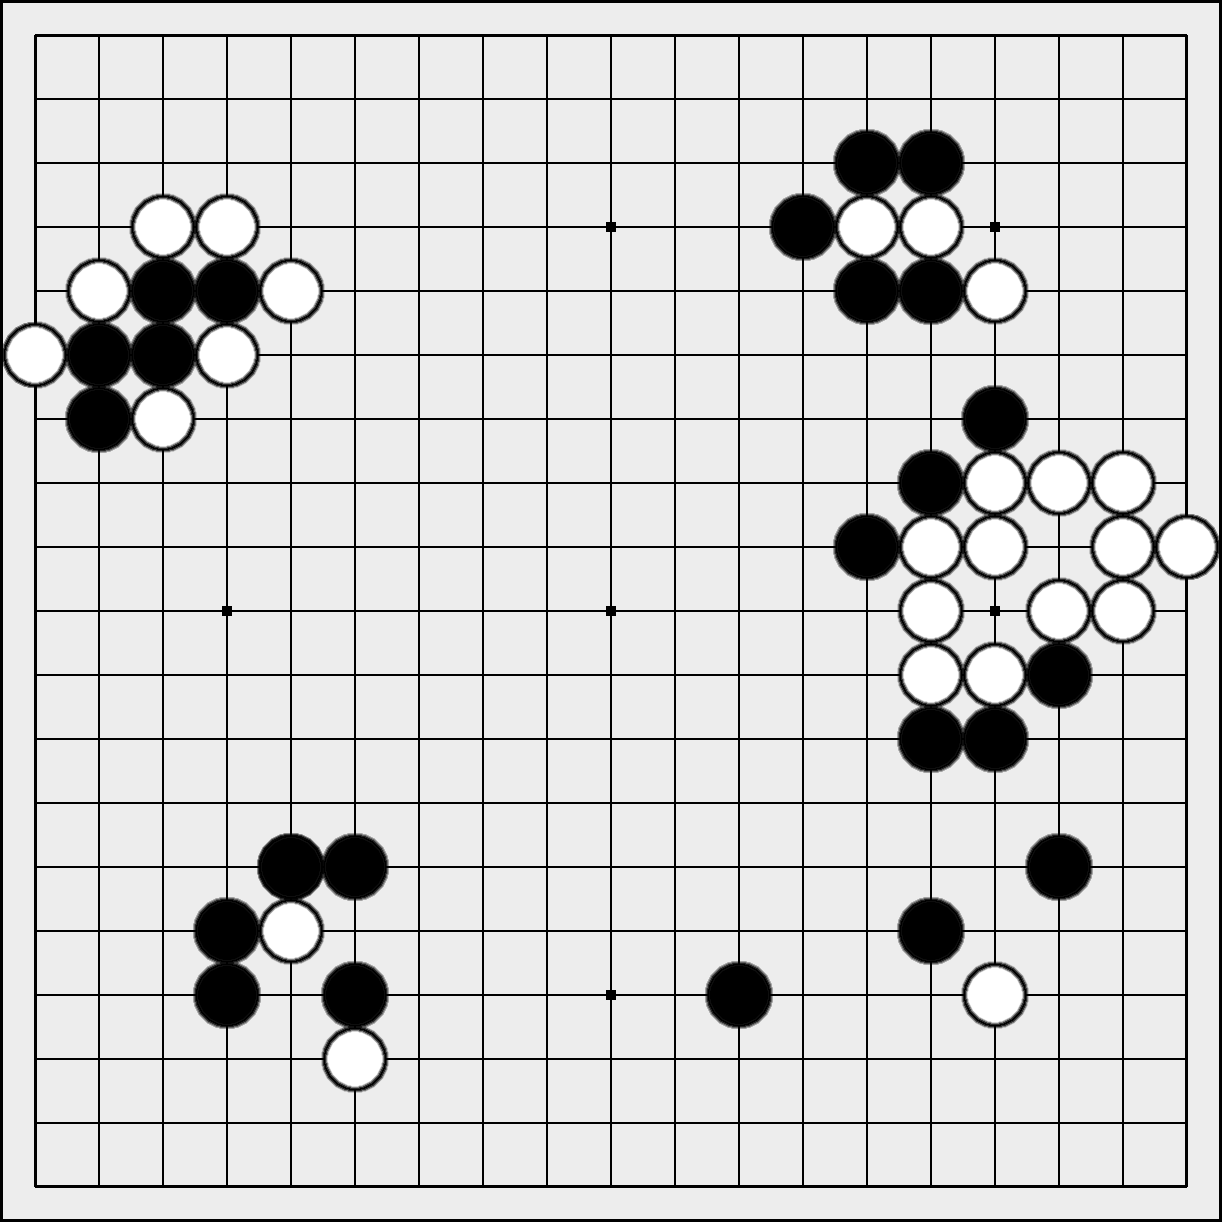
\includegraphics[width = 0.8 \textwidth]{go_illustration.png}

\caption{$19 \times 19$ Go-lauta ja kärjistetty pelitilanne. Vasemmalla ylhäällä valkea on ympäröinyt mustan kiviä tikapuiksi kutsuttuun muodostelmaan. Oikealla ylhäällä valkean kaksi kiveä ovat vangittavissa yhdellä siirrolla eli \textit{atarissa}. Oikealla keskellä valkea on muodostanut ryhmän, jolla on kaksi silmää, eli mustan yritys vangita ryhmä ympäröimällä ei voi onnistua. Todellisessa pelissä syntyvät muodostelmat ovat yleensä monimutkaisempia.}
\end{figure}

\subsection{Gon esittely}

Go on kombinatorinen lautapeli, jota on pelattu Aasiassa jo yli kahdentuhannen vuoden ajan. Pelissä kaksi pelaajaa asettaa vuorotellen pelilaudan ruudukon risteyksiin kiviksi kutsuttuja pelinappuloita tarkoituksenaan vallata pelilaudan alueita ja vangita vastustajan kiviä ympäröimällä ne omillaan. Pelin voittaja määräytyy pelaajien hallitseman alueen ja vastustajiltaan poistettujen kivien määrän perusteella.

Go-lautoja on erikokoisia, mutta virallisissa kilpailuissa käytetään $19 \times 19$ -risteyksen lautaa. Näin isolla laudalla pelit kestävät tyypillisesti satoja vuoroja, ja kullakin vuorolla mahdollisia siirtoja on keskimäärin noin 250~\cite{browne}. Pelipuu on siis kohtuuttoman suuri käsiteltäväksi perinteisellä minimax-haulla. Gohon on myös vaikea kehittää vahvoja heuristiikkoja, sillä yksittäisten kivien tai kiviryhmien arvo pelaajalle voi riippua paljon pelilaudan kokonaistilanteesta tai tulla ilmeiseksi vasta paljon myöhemmin pelissä.
\newpage
MCTS on suosittu menetelmä go-tekoälyissä. Menetelmää sovellettiin peliin ensimmäistä kertaa vuonna 2006, ja ammattilaispelaajan pienellä $9 \times 9$ -laudalla voittava MCTS-tekoäly esiteltiin vuonna 2008~\cite{browne}. MCTS toimii gossa perinteisiä minimax-menetelmiä paremmin, sillä sen simulaatioon perustuva lähestymistapa ei tarvitse heuristiikkaa ja havaitsee siirtojen pitkän aikavälin vaikutuksia automaattisesti simulaatiovaiheessaan. Parhaita tuloksia saavuttavat tekoälypelaajat eivät kuitenkaan käytä pelkkää MCTS:ää, vaan yhdistävät menetelmään perinteisen tekoälyn piirteitä~\cite{browne}.

\subsection{AMAF-heuristiikka}

Parhaat gon tekoälypelaajat käyttävät siirtokohtaista odotusarvoa (\textit{All moves as first}, jatkossa AMAF)~\cite{browne}. AMAF-menetelmässä pelipuun solmut mallintavat siirtoja kokonaisten pelitilanteiden sijaan. Koska samat siirrot johtavat kombinatorisessa pelissä aina samaan tilanteeseen, tämä malli on yhtäpitävä tavallisen pelipuun kanssa. Tavallisen UCT:n tapaan AMAF valitsee osittaisesta pelipuusta laajennettavan solmun ja simuloi solmun kuvaamasta pelitilanteesta pelin lopputilaan asti saaden lopputulosta kuvaavan $\Delta$-arvon.

Toisin kuin tavallinen UCT, AMAF päivittää solmujen odotusarvoja $\Delta$:n avulla vaikka ne pelattaisiin myöhemmin simulaatiossa~\cite{browne, helmbold}. AMAF-heuristiikka siis olettaa siirtojen hyödyn pelaajalle olevan osittain pelitilanteesta riippumattomia. Tämä oletus lisää siirtojen laskemia simulaatiokertoja suorittamatta todellisuudessa enempää simulaatioita, joten solmujen odotusarvo kehittyy nopeasti. Odotusarvo voi kuitenkin kehittyä harhaanjohtavaksi siirroille, joiden arvo riippuu paljon muusta pelitilanteesta~\cite{helmbold}.

AMAF:stä on useita muunnelmia, kuten $\alpha$-AMAF joka käyttää painokerrointa $\alpha$ painottaakseen solmun odotusarvon kertymistä. Kukin solmu saa lopulliseksi odotusarvokseen
\begin{equation}
\alpha A + (1 - \alpha)U
\end{equation}
missä $A$ on solmun odotusarvo sen kautta simuloiduista peleistä ja $U$ on solmun normaali UCT:n mukainen odotusarvo. Erityisen suosittu AMAF-muunnelma on RAVE (\textit{Rapid Action Value Estimation}), joka toimii kuten $\alpha$-AMAF, mutta pienentää $\alpha$:n arvoa solmun vierailukertojen mukaan. Tämä heuristiikka saa nopeasti karkeita arvioita, mutta vaihtaa hitaasti edetessään painotustaan kohti tarkempaa, tavallista UCT:tä~\cite{browne}.

\subsection{Pelitilanteeseen pohjautuvat heuristiikat}

Gossa tilannetta, jossa kiviryhmä on vaarassa joutua vangiksi vastustajan seuraavalla siirrolla, kutsutaan \textit{atariksi}. Cazenave ym.~\cite{cazenaveatari} esittelevät heuristiikan, joka vaikuttaa lopulliseen solmun valintaan painottaen siirtoja jotka asettavat vastustajan kiviryhmän atariin tai vapauttavat omia kiviryhmiä atarista. Vastaavasti heuristiikka välttää siirtoja, jotka johtavat omien kiviryhmiensä joutumista atariin. Suurempien kiviryhmien atareja painotetaan enemmän kuin pienien.

Toinen Cazenaven ym.~\cite{cazenave} käyttämä heuristiikka laskee kiviryhmien sisällä olevia vapaita risteyksiä, joita kutsutaan kiviryhmän silmiksi. Kiviryhmää, jolla on vähintään kaksi silmää, ei voi vangita, sillä vastustajan pelatessa silmään hänen oma kivensä tulee välittömästi vangituksi. Koska silmät ovat erittäin arvokkaita kiviryhmien turvaamisessa, Cazenaven ym. heuristiikka karsii pois siirrot jossa pelaaja poistaisi itseltään silmiä.

Wang ja Gelly~\cite{wanggelly} esittelevät simulaatiovaiheen heuristiikan, joka etsii laudalta tiettyjä $3\times 3$ risteyksen kuvioita etukäteen koottuun kuviokirjastoon pohjautuen. Kuviokirjaston avulla laudalta etsitään tiettyjä tilanteita, jotka on pelikokemuksen myötä havaittu erityisen tärkeiksi. Tällaisia tilanteita ovat mm. kahden yhdistymistä tavoittelevan vastustajan kiviryhmän katkaiseminen keskeltä.

Kuten Cazenaven atari-heuristiikka, Wangin ja Gellyn menetelmä pyrkii ensisijaisesti pelastamaan omia kiviryhmiään atarista simulaatiovaiheessa. Jos tälle ei ole tarvetta, heuristiikka etsii viimeksi pelaamansa siirron läheltä mahdollisuuksia toteuttaa sille annettun kuviokirjaston määrittelemiä kuvioita~\cite{wanggelly}. Kuvioheuristiikka on yksi tapa tuottaa vahvoja pelejä simulaatiovaiheessa ja paransi Wangin ja Gellyn tekoälyn voittosuhdetta kolmellakymmenellä prosenttiyksiköllä~\cite{wanggelly}.


\subsection{Ajanhallinta}

Gota pelataan turnauspeleissä usein pelikellon kanssa. Pelin voi hävitä normaalin lopputilanteen lisäksi käyttämällä vuoroihinsa liikaa aikaa, joten mietintäajan hajauttaminen oikein on erityisen tärkeää. Huang ym.~\cite{huang} tutkivat artikkelissaan gon ajanhallintaa MCTS:n yhteydessä tarkoituksenaan jakaa jäljellä oleva peliaika mahdollisimman tehokkaasti jäljellä olevaa peliä varten.

Yksinkertaisin peliajan jakamisen malli on varata kullekin vuorolle aikaa samassa suhteessa jäljellä olevaan aikaan nähden~\cite{huang}. Menetelmä antaa ensimmäiselle vuorolle eniten aikaa, ja sen jälkeen kullekin vuorolle vähemmän jäljellä olevan ajan mukaan. Koska MCTS:n simulaatiovaiheet suoritetaan nopeammin lähempänä loppupeliä, vuorojen lyheneminen ei ole suuri haitta. Alkupelin vuoroille annetaan kuitenkin enemmän aikaa kuin mitä niihin tarvittaisiin, ja tämän ajan voisi käyttää tehokkaammin pelin keskivaiheilla jolloin merkittäviä siirtoja tapahtuu enemmän.

Huangin ym. vaihtoehtoinen ratkaisu määrittää vuorolle $n$ annetun mietintäajan $t_n$ lausekkeella
\begin{equation}
t_n = \frac{t}{C + \max(n_{max} - n, 0)}\,,
\end{equation}
missä $t$ on jäljellä oleva peliaika, ja $C$ sekä $n_{max}$ ovat vakioita~\cite{huang}. Tämä ratkaisu antaa vähemmän aikaa alkupelille mutta kasvattaa kunkin vuoron käyttämää ajan määrää kunnes saavutetaan vuoro $n_{max}$, mistä eteenpäin kunkin vuoron osuus jäljellä olevasta peliajasta pysyy vakiona. Huangin ym. go-tekoälyn voittoprosentti parani keskipeliä painottavalla ajanhallinnalla kuusi prosenttiyksikköä~\cite{huang}.

On mahdollista, että UCT-haun päättyessä eniten tutkittu solmu on eri kuin solmu, jolla on korkein odotusarvo. Tällainen tilanne aiheutuu usein, kun eniten vieraillun solmun odotusarvo on laskussa tai haun loppuvaiheissa löydetään uusi, kannattavampi haara~\cite{huang}. Saadakseen selville mikä solmu on todella paras, Huangin ym. tekoäly jatkaa hakua antamalla sille ylimääräistä hakuaikaa puolet sen alkuperäisestä hakuajasta. Laskennan kohdennettu pidentäminen vähentää myöhempien siirtojen peliaikaa, mutta parantaa Huangin ym. kokeiden mukaan voittoprosenttia seitsemällä prosenttiyksiköllä~\cite{huang}.

Huang ym. esittelevät algoritmiin muutoksen, joka antaa UCT:n jatkaa hakua ylimääräisellä laskenta-ajalla jos juurisolmun odotusarvo on haun lopuksi jotain määriteltyä kynnysarvoa pienempi~\cite{huang}. Ajatuksena on saada UCT miettimään tavallista tarkemmin tilanteissa, joissa ajan loppumisen sijaan ollaan häviämässä huonon pelitilanteen takia. Lisäajan antaminen häviöllä olevalle algoritmille parantaa Huangin ym. tutkimuksissa algoritmin voittoprosenttia edelliseen heuristiikkaan yhdistettynä noin viidellä prosenttiyksiköllä~\cite{huang}.

Pohdiskelulla (\textit{pondering}) tarkoitetaan pelitilanteen laskentaa vastustajan vuorolla~\cite{huang}. Menetelmän tarkoituksena on hyödyntää tehokkaasti vastustajan laskenta-aikaa. Yksinkertaisin MCTS:n kanssa käytetty pohdiskelumenetelmä on suorittaa MCTS-algoritmia vastustajan vuorolla kuin olisi tekoälyn vuoro. Kun vastustaja tekee siirtonsa, pohdiskellessa rakennetusta pelipuusta valitaan vastustajan siirron mukainen haara ja aloitetaan vuoron MCTS-haku käyttäen sitä pohjana.

Pohdiskelun voi kohdistaa koko mahdollisten siirtojen joukon sijasta vain tietyihin siirtoihin, joita tekoäly arvioi vastustajan tekevän~\cite{huang}. Pohdiskeltavat siirrot valitaan omalla vuorolla suoritetun UCT:n perusteella, ja pohdiskellessa suoritettava UCT tutkii vain valittuja siirtoja. Huangin ym. havaitsivat vastustajan tekemän siirron kuuluvan pohdiskelualgoritmin valitsemiin siirtoihin vain n. 57\% kerroista, ja tulosten olevan voittoprosentin kannalta samaa tasoa kuin yksinkertaisemmalla pohdiskelualgoritmilla~\cite{huang}.

Koska myös vastapelaajan voi olettaa pohdiskelevan, kannattaa pohdiskelevan tekoälyn pyrkiä pelaamaan mahdollisimman lyhyitä vuoroja paitsi säästääkseen omaa aikaansa, myös evätäkseen vastustajalta ylimääräisen laskenta-ajan pohdiskeluun~\cite{huang}. Nopeilla siirroilla voi saavuttaa suurta hyötyä, sillä vähän pohdiskelemaan ehtivä vastustaja joutuu hyvään tulokseen päästäkseen laskemaan enemmän omalla vuorollaan, jolloin tekoäly saa enemmän pohdiskeluaikaa. 

Pohdiskelun perusteella nopeasti pelaaminen on mahdollista, kun tekoälyn pohdiskellessa suorittamat simulaatiot osuvat paljon siihen osaan pelipuuta, jonka vastustaja valitsee~\cite{huang}. Huangin ym. tekoäly laskee vuoronsa aluksi, kuinka iso osa simulaatiokerroista suoritettiin pelipuun osassa jonka vastapelaaja valitsi. Tekoäly saa vuoroaan varten normaalin laskenta-aikansa vähennettynä vastapelaajan vuoron pituuteen kerrottuna oikein osuneiden simulaatioiden osuudella. Nopeutettua pelaamista käyttävä menetelmä voitti Huangin ym. kokeissa vastaavan tavallisen pohdinnan 52\% peleistä~\cite{huang}.

\section{Rinnakkaistettu MCTS}

MCTS on mahdollista rinnakkaistaa siten, että algoritmi suorittaa useita simulaatioita samanaikaisesti~\cite{browne, cazenave}. Rinnakkaistaminen nopeuttaa valmiiden simulaatiotulosten kertymistä, jolloin tekoälyn kilpailukyky kasvaa laskenta-ajan pysyessä samana. Rinnakkaistamisessa on kuitenkin haasteena eriytettyjen laskentasäikeiden välinen tahdistus ja viestintä.

Chaslot ym.~\cite{chaslot} luettelevat kolme keskeistä menetelmää MCTS:n rinnakkaistamiseen. Cazenaven ym.~\cite{cazenave} go-tekoälyjä varten kehittämä lehtirinnakkaistaminen on malleista yksinkertaisin. Lehtirinnakkaistetussa MCTS:ssä laajennettava solmu valitaan sarjallisesti, mutta siitä suoritetaan useita rinnakkaisia simulaatioita jotka valitsevat omat polkunsa pelin loppuun. Menetelmä on yksinkertainen toteuttaa eikä vaadi muistialueiden suojaamista samanaikaiselta käsittelyltä.

Lehtirinnakkaistamisen heikkoutena on, että eri säikeet voivat suorittaa simulaationsa loppuun eri tahdissa~\cite{chaslot}. Koska pelipuuta laajennetaan vasta kun kaikki simulaatiot on suoritettu loppuun, simulaatiovaihe kestää yhtä kauan kuin hitaimman säikeen simulaatio. Loppuun päässeet säikeet puolestaan odottavat toimettomina. Suorituskyky ei siis parane mielivaltaisen paljon säikeiden määrää lisäämällä.

Puurinnakkaistaminen on Chaslotin ym. esittelemä rinnakkaistamismenetelmä, joka suorittaa samanaikaisia MCTS-prosesseja samalle pelipuulle~\cite{chaslot}. Lehtirinnakkaistamisesta poiketen puurinnakkaistamisen säikeet suorittavat koko MCTS-algoritmin pelkän simulaatiovaiheen sijaan. Koska useampi hakusäie käsittelee samaa puuta, täytyy estää enempää kuin yhtä säiettä kerrallaan pääsemästä käsiksi varsinaiseen pelipuuhun. Vain yksi säie kerrallaan voi siis laajentaa pelipuuta tai päivittää pelipuun solmujen arvoja simulaatiotuloksilla.

Jos pelin kesto on pitkä ja simulaatiovaihe kestää vastaavasti kauan, ei varsinaisen pelipuun käytön rajaaminen ole kovin ongelmallista. Jos säikeet palaavatkin simulaatiovaiheesta usein puuhun, voi puun rajaaminen yhdelle säikeelle muodostua pullonkaulaksi~\cite{chaslot}. Vaihtoehtoisesti puuhun voi päästä useampia säikeitä niin, että jokainen pelipuun solmu rajataan vain yhden säikeen käyttöön kerrallaan. Tämä kuitenkin vaatii tiheää solmujen lukitsemista ja avaamista, johon kuluu ylimääräistä laskenta-aikaa.

Puurinnakkaistamisen heikkouksiin kuuluu sen liiallinen keskittyminen samoihin hakupolkuihin~\cite{browne, chaslot}. Koska kaikki hakusäikeet käyttävät samaa puuta ja UCT suosii solmuja joista on saatu lupaavia tuloksia, säikeet tutkivat usein pientä osaa puusta todella tarkasti laajemman tiedustelun sijaan. Coulom ehdottaa ongelmaan ratkaisuksi tilapäistä sakkoarvoa (\textit{virtual loss}), jonka säie jättää solmuun kulkiessaan sen läpi~\cite{chaslot}. Tämä saa toiset säikeet suosimaan muiden solmujen tutkimista mutta ei poissulje selvästi ylivertaisen solmun tutkimista usean säikeen voimin.

Juuririnnakkaistaminen on Cazenaven ym.~\cite{cazenave} kehittämä MCTS:n rinnakkaistusalgoritmi, joka suorittaa puurinnakkaistamisen tapaan täyden MCTS-algoritmin jokaisessa säikeessä. Juuririnnakkaistettu MCTS tuottaa pelimetsän antamalla jokaiselle säikeelle oman pelipuun, jolloin poistuu puurinnakkaistamisen tarve suojata muistia samanaikaiselta käytöltä. Kun laskenta-aika on käytetty loppuun, valitaan pelipuiden tuottamien tulosten mukaan pelattava siirto.

Perinteinen ratkaisu pelattavan siirron valintaan pelimetsän perusteella on valita pelipuissa yhteenlasketusti eniten tutkittu solmu~\cite{browne}, mutta Soejima ym.~\cite{soejima} esittelevät vaihtoehtoisen strategian, jossa siirto valitaan enemmistöäänestyksellä. Enemmistöäänestys valitsee siirron, joka on useimman pelipuun eniten vierailtu solmu, eikä siten joudu tilanteisiin joissa metsän suosikiksi valitaan mielummin kaikkien toisiksi parhaana pitämä strategia kuin siirto, joka on enemmistön mielestä paras~\cite{soejima}.


\section{MCTS ei-kombinatorisissa peleissä}

\subsection{Epätäydellinen informaatio ja satunnaisuus}

Epätäydellisen informaation peli on peli, jossa kaikki pelaajat eivät tiedä kaikkea vallitsevasta pelitilanteesta~\cite{browne}. Esimerkiksi pokerissa kukin pelaaja näkee vain oman kätensä kortit. Monessa pelissä pelitilanteeseen vaikuttavat myös satunnaistekijät, kuten nopanheitot. MCTS on erilaisten apukeinojen avulla sovellettavissa myös peleihin, joissa informaatio on epätäydellistä ja osa pelitilanteesta määräytyy satunnaistekijöiden kautta~\cite{browne}.

Determinisaatiolla tarkoitetaan satunnaisuutta tai epätäydellistä informaatiota sisältävän pelin analysointia käsittelemällä sitä deterministisen pelin tavoin~\cite{browne}. Determinisoitavasta pelitilanteesta luodaan mahdollisia pelitilanteita, joissa kaikki informaatio on pelaajille avointa ja satunnaistekijöiden arvot on kiinnitetty tunnetuiksi. Nämä pelitilanteet kuvaavat mahdollisia tilanteita eri satunnaistilojen ja piilotetun informaation arvoille. Niihin voidaan soveltaa kombinatorisen pelin MCTS-menetelmää, ja saatuja tuloksia voidaan käyttää toimintamallin valitsemiseen alkuperäisessä epädeterministisessä pelissä.

Vastustajan strategian mallintaminen on erityisen tärkeää, kun pelin informaatio on epätäydellistä~\cite{browne}. Ainoastaan vastustajan tiedossa oleva informaatio voi vaikuttaa tämän tekemiin siirtoihin, jolloin vastustajan strategiasta voi muodostaa johtopäätöksiä vain tämän tiedossa olevasta informaatiosta. Esimerkiksi Ponsen ym.~\cite{ponsen} käyttivät pokerissa vastustajan mallinnusta Bayes-relaatiomalleilla päätelläkseen vastustajan kädessä olevien korttien todennäköisyysjakauman ja hyödynsivät tuloksia determinisoitujen pelien luomisessa MCTS:ä varten.

\subsection{Videopelit}

Reaaliaikaisessa pelissä pelitilanne voi edetä, vaikka pelaaja ei toimisi mitenkään~\cite{browne}. Tämä pakottaa pelaajan toimimaan erityisen nopeasti, sillä liian pitkään mietitty siirto voi muuttua harkinnan aikana huonoksi tai laittomaksi. Useimmat reaaliaikaiset pelit ovat videopelejä, joissa esiintyy lisäksi muitakin haasteita kuten satunnaisuutta, informaation epätäydellisyyttä ja erityisen suuria määriä mahdollisia pelitilanteita.

Samothrakis ym.~\cite{samothrakis} tutkivat MCTS-pohjaisen menetelmän toimintaa \textit{Ms. Pac-Man} -pelissä. Pelissä pelaaja kuljettaa hahmoa sokkelossa tarkoituksenansa kerätä kartalla olevat pisteet ja vältellä vihollisia. Vastapelaajina on neljä vihollista, joiden osittain satunnainen tekoäly pyrkii nappaamaan pelihahmon. Pelissä ei ole suoranaisia lopputiloja paitsi pelaajan hävitessä, joten MCTS:n simulaatiovaiheen täytyy rajata haku muilla tavoin. Samothrakis ym. ratkaisi ongelman rajaamalla simulaation maksimisyvyyden ja käyttämällä haun katkaisusolmun arviointiin yksinkertaista heuristiikkaa.

Toinen haaste \textit{Ms. Pac-Man} -pelissä on ajoituksen tarkkuus. Samothrakis ym. toteaa, että peli vaatii siirtojen tapahtuvan jopa 50-60 millisekunnin tarkkuudella, mikä asettaa tiukan rajan pelipuussa suoritettavan simulaation määrälle. Tulokset havaittiin kuitenkin erittäin hyviksi, ja MCTS-menetelmällä toimiva tekoäly keräsi testeissä evolutionaarisia ja geneettisiä algoritmeja sekä vahvistusoppimista hyödyntäviä menetelmiä kahta kertaluokkaa paremmat pisteet~\cite{samothrakis}.

\textit{Warcraft 2} on reaaliaikainen strategiapeli, jossa pelaajat rakentavat itselleen tukikohtia ja ohjaavat armeijoita tarkoituksenaan tuhota vastapelaajien joukot ja tukikohdat. Tekoälylle erityisiä haasteita pelissä ovat reaaliaikaisuus, epätäydellinen informaatio ja erittäin suuri mahdollisten siirtojen määrä. Balla ym.~\cite{balla} tutkivat sotilasyksiköiden koordinoimista tehokkaiksi hyökkäysjoukoiksi yksittäisiä taisteluita varten \textit{Warcraft 2}:ssa.

Balla ym. havaitsivat, että erilaisten pelitilanteiden monipuolisuus tekee vaikeaksi löytää UCT:n tutkimusvakiolle $C_p$ yleisesti hyvää arvoa~\cite{balla}. Ongelma ratkaistiin käyttämällä tutkimusvakiona tilan odotusarvoa. Koska jokaista sotilasyksikköä voi komentaa erikseen muista riippumatta ja armeijat voivat olla kymmenien yksiköiden suuruuksia, hakuavaruutta pienennettiin abstrahoimalla yksittäiset sotilasyksiköt joukoiksi, jotka vastaanottavat yhteisiä käskyjä ja pitävät yllä tietoa yksiköidensä kunnosta, sijainnista ja tilasta.

Ballan ym. käyttämässä hakupuussa kukin solmu ylläpitää tietoa kaikkien pelaajien sotilasjoukoista, omien joukkojen tämänhetkisestä toiminnasta ja peliajasta~\cite{balla}. Kukin yksittäinen siirto pelipuussa antaa käskyn yhdelle omalle joukolle, joka ei vielä tee mitään. Käsky voi olla esimerkiksi yhdistää joukko toiseen, siirtää joukkoa tai saattaa joukko taistelemaan vihollissotilaiden kanssa.

\section{Yhteenveto}

MCTS:n vahvuus on sen helppo sovellettavuus erilaisiin ongelmiin~\cite{browne}. Koska se ei tarvitse heuristiikkaa, tekoälyn ohjelmoijan ei tarvitse tietää pelattavasta pelistä muuta kuin perussäännöt. Heuristiikan tarpeettomuus mahdollistaa MCTS:n tehokkaan käytön myös peleihin, joihin ei tunneta hyviä heuristiikkoja.

Useat MCTS-toteutukset, kuten UCT, kohdistavat haun tehokkaasti ja laajentavat pelipuuta eniten suuntiin, joista on saatu lupaavimpia tuloksia~\cite{browne}. Näin algoritmi ei käytä paljoa aikaa huonoja tuloksia antaneiden vaihtoehtojen tutkimiseen. UCT takaa kuitenkin, että kukin solmu valitaan laajennettavaksi nollaa suuremmalla todennäköisyydellä. On siis erittäin epätodennäköistä, että yksittäiset huonot kokemukset estävät algoritmia löytämästä todellisuudessa hyviä strategioita.

Parhaita tuloksia MCTS:n käytössä pelitekoälyissä saadaan yhdistämällä perusmenetelmään pelikohtaisia parannuksia. Esimerkiksi gossa tasokkaimmat MCTS-pohjaiset tekoälyt käyttävät AMAF-heuristiikkaa, kuviokirjastoja tai muita pelitekoälyssä yleisiä tekniikoita parantaakseen suoritustaan~\cite{browne}. MCTS-menetelmän saa sopivilla muunnelmilla toimimaan tehokkaasti myös ei-kombinatorisissa peleissä.

MCTS ylläpitää arviota siirtojen kannattavuudesta reaaliaikaisesti. Haun voi siis keskeyttää koska tahansa ja saada silti kelvollisen ratkaisun. Pidemmän laskenta-ajan antaminen MCTS:lle parantaa kuitenkin tuloksen laatua, sillä algoritmilla on enemmän aikaa suorittaa simulaatioita ja parantaa niiden avulla arvioitaan siirtojen kannattavuudesta~\cite{browne}.


% --- References ---
%
% bibtex is used to generate the bibliography. The babplain style
% will generate numeric references (e.g. [1]) appropriate for theoretical
% computer science. If you need alphanumeric references (e.g [Tur90]), use
%
% \bibliographystyle{babalpha-lf}
%
% instead.

\bibliographystyle{babplain-lf}
\bibliography{lahteet}


% --- Appendices ---

% uncomment the following

% \newpage
% \appendix
% 
% \section{Esimerkkiliite}

\end{document}

